\documentclass{standalone}

\begin{document}

\setbeamerfont{block body}{size=\scriptsize}
\setbeamerfont{block body example}{size=\scriptsize}
\setbeamerfont{block body alerted}{size=\scriptsize}
\setbeamertemplate{itemize/enumerate body begin}{\scriptsize}
\setbeamertemplate{itemize/enumerate subbody begin}{\scriptsize}

\begin{frame}{The Big Data era}{Biological Big Data}

  \setbeamercolor{block title example}{bg=white, fg=DarkGreen}
  \setbeamercolor{block body example}{bg=white, fg=black}

  \scriptsize{Considering the annual growth of data generation, the digital universe (i.e. data we generate annually) will reach 44 zettabytes by the year 2020, which is ten times the size of the digital universe in 2013. This trend in rising data volume is supported by:}

  \begin{figure}
    \centering
    \includegraphics[width=.5\linewidth]{grow.jpg}
  \end{figure}

  \begin{exampleblock}{Single Sequenced Human Genome}
    The size of a single sequenced human genome is approximately 200 Gb for less than US \$ \numprint{1000} (National Human Genome Research Institute, 2016).
  \end{exampleblock}

  \begin{exampleblock}{Datasets available online}
    The amount of available data from large project such as \numprint{1000} Genomes (\url{http://www.1000genomes.org}) will collectively approach the petabyte scale for the raw information alone.
  \end{exampleblock}

\end{frame}



\begin{frame}{A new research paradigm}{Biological Big Data}

  \setbeamertemplate{itemize items}[ball]

  \begin{columns}

    \begin{column}{0.5\textwidth}

      The problems concerning the Big Data Analytics must be faced on two fronts:

      \vspace{0.6cm}
      \textbf{Algorithm and Models:}

      \begin{itemize}

        \item Data visualization
        \item Dimensionality reduction
        \item Parallel computing
        \item Optimization

      \end{itemize}

    \end{column}
    \begin{column}{0.5\textwidth}

      \begin{figure}
        \centering
        \includegraphics[width=.8\linewidth]{h2020.jpg}
      \end{figure}

      \textbf{Hardware and Technology:}

      \begin{itemize}

        \item HPC
        \item Cloud
        \item Storage
        \item Data exchange

      \end{itemize}

    \end{column}
  \end{columns}

  \vspace{0.5cm}

  A \textbf{new paradigm} is emerging and it needs new hybrid sciences as Bioinformatics, Computational Sociology and new hybrid tools as Hybrid Cloud Architecture, Data Mining Algorithms.

\end{frame}


\begin{frame}{Biological features}{Gene expression Big Data}

  \setbeamertemplate{itemize items}[ball]

  \begin{columns}

    \begin{column}{0.4\linewidth}

      \begin{figure}[htbp]
        \centering
        \def\svgwidth{0.8\linewidth}
        \input{./img/distributions.pdf_tex}
      \end{figure}

    \end{column}
    \begin{column}{0.6\linewidth}

      \begin{itemize}
        \item single parameter classification fails in predicting higher dimension classification performance;

        \item feature1 and feature2 classify badly in 1D, but have a very good performance in 2D;

        \item Activity of a biological feature as a function of its expression level: monotonically increasing; "windowed" behavior.

      \end{itemize}

    \end{column}
  \end{columns}

  \begin{figure}[htbp]
    \centering
    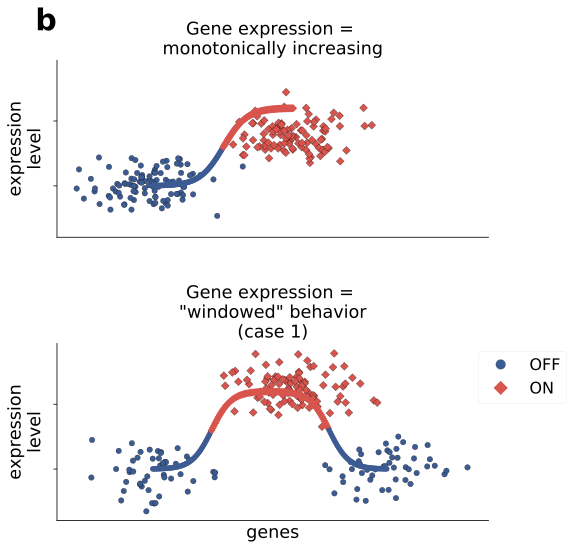
\includegraphics[width=0.9\linewidth]{expression.png}
  \end{figure}

\end{frame}


\begin{frame}{Classification and dimensionality reduction}{DNetPRO algorithm}

  \setbeamertemplate{itemize items}[ball]

  The potential clinical utility of genomic, transciptomic, epigenomic and proteomic data in aggregate remains largely unknown.

  The goal of these type of analyses is to identify the \textbf{smallest number of probes} able to hold the most information about classes.

  \vspace{.5cm}

  \textbf{DNetPRO} (Discriminant analysis with Network PROcessing) algorithm:

  \vspace{1cm}

  \begin{columns}

    \begin{column}{0.5\linewidth}

      \textbf{Computational Field:}

      \begin{itemize}
        \item Feature selection
        \item Dimensionality reduction
        \item Classification
      \end{itemize}

    \end{column}

    \begin{column}{0.5\linewidth}

      \textbf{Biological Field:}

      \begin{itemize}
        \item Evaluation of genes interaction
        \item Easy interpretation
        \item Extraction of Signature
      \end{itemize}

    \end{column}

  \end{columns}

\end{frame}

%% OPTIMIZATIONS

\begin{frame}{DNetPRO algorithm}{Pipeline description}

  \begin{figure}
    \begin{overprint}
      \onslide<1>\centering\includegraphics[width=0.8\linewidth]{pseudo_dnet.png}
      \onslide<2>\vspace{1cm}\centering\includegraphics[width=\linewidth]{dnet_pipe.png}
    \end{overprint}
  \end{figure}

\end{frame}


\begin{frame}{DNetPRO algorithm}{Algorithm optimization}

  Porting on a parallel environment: \textsf{C++} multi-threading implementation for network construction.

  Distributed computation of each pipeline step (\textsf{snakemake}).

  \begin{columns}

    \begin{column}{0.5\linewidth}

      \begin{figure}[htbp]
        \centering
        \def\svgwidth{0.8\linewidth}
        \input{./img/samples_timing.pdf_tex}
      \end{figure}

    \end{column}

    \begin{column}{0.5\linewidth}

      \begin{figure}[htbp]
        \centering
        \def\svgwidth{0.8\linewidth}
        \input{./img/features_timing.pdf_tex}
      \end{figure}

    \end{column}

  \end{columns}

    \begin{figure}[htbp]
      \centering
      \def\svgwidth{0.5\linewidth}
      \input{./img/nth_timing.pdf_tex}
    \end{figure}

\end{frame}

\begin{frame}{DNetPRO algorithm}{Algorithm optimization}

  Porting on a parallel environment: \textsf{C++} multi-threading implementation for network construction.

  Distributed computation of each pipeline step (\textsf{snakemake}).

  \begin{figure}
    \centering
    \includegraphics[width=\linewidth]{qdanet_pipe_single.png}
  \end{figure}

\end{frame}

%% APPLICATIONS

\begin{frame}{DNetPRO algorithm}{Applications}

  \setbeamertemplate{itemize items}[ball]

  \begin{columns}

    \begin{column}{0.5\textwidth}

      \begin{exampleblock}{Synthetic dataset}
          Study of the characteristics of the algorithm with different number of samples and features.

          \begin{figure}
            \centering
            \def\svgwidth{0.8\linewidth}
            \input{./img/features_toy.pdf_tex}
          \end{figure}

      \end{exampleblock}

    \end{column}
    \begin{column}{0.5\textwidth}

      \begin{block}{Cytokinome dataset}
        \begin{itemize}
          \item Study on Alzheimer's disease;
          \item 26 cytokine expression levels;
          \item 289 subjects (189 female and 100 male);
        \end{itemize}
      \end{block}

      \begin{alertblock}{Bovine dataset}
        \begin{itemize}
          \item Study on Paratuberculosis disease;
          \item 15 mRNA samples of 3 bovine classes;
          \item 13529 features each;
        \end{itemize}
      \end{alertblock}

    \end{column}

  \end{columns}

  \setbeamercolor{block title alerted}{fg=black, bg=orange!40!white}
  \setbeamercolor{block body alerted}{fg=black, bg=orange!20!white}

  \begin{alertblock}{Benchmark state-of-art}

    \begin{columns}
      \begin{column}{0.4\linewidth}

        \begin{itemize}
          \item Application on Synapse dataset;
          \item mRNA, miRNA and RPPA samples;
        \end{itemize}

      \end{column}
      \begin{column}{0.6\linewidth}

        \begin{itemize}
          \item 4 different tumors\\(KIRC, GBM, LUSC and OV);
          \item benchmark on state-of-art\\(Yuan et al., \emph{Nature methods}, 2014);
        \end{itemize}
      \end{column}
    \end{columns}

  \end{alertblock}

\end{frame}




\begin{frame}{Synapse dataset}{DNetPRO benchmark}

  \setbeamertemplate{itemize items}[ball]

  \begin{columns}

    \begin{column}{0.5\linewidth}
      \textbf{TCGA} dataset - The Cancer Genome Atlas

      \vspace{0.5cm}

      \textbf{Dichotomization:} normal/tumor
    \end{column}

    \begin{column}{0.5\linewidth}
      \begin{figure}
        \centering
        \includegraphics[width=\linewidth]{synapse_table.png}
      \end{figure}
    \end{column}

  \end{columns}

  \vspace{1cm}

  \begin{columns}

    \begin{column}{0.6\linewidth}

    4 cancer types:

    \begin{itemize}
      \item KIRC (\emph{Kidney Renal clear cell Carcinoma})
      \item GBM (\emph{Glioblastoma Multiforme})
      \item LUSC (\emph{Lung Squamous Cell Carcinoma})
      \item OV (\emph{Ovarian serous cystadenocarcinoma})
    \end{itemize}

    \end{column}

    \begin{column}{0.4\linewidth}

      3 molecular data types:

      \begin{itemize}
        \item mRNA
        \item miRNA (\emph{micro RNA})
        \item RPPA (\emph{Reverse Phase Protein Array})
      \end{itemize}

    \end{column}

  \end{columns}

\end{frame}




\begin{frame}{Synapse dataset}{mRNA Results}

  \scriptsize{Benchmark with 8 classifiers with different features selection methods: \textbf{DDA} (diagonal discriminant analysis); \textbf{KNN} (K-nearest neighbor); \textbf{DA} (discriminant analysis); \textbf{LR} (logistic regression); \textbf{NC} (nearest centroid); \textbf{PLS} (partial least squares); \textbf{RF} (random forest); \textbf{SVM} (support vector machine).}

  \begin{figure}
    \begin{overprint}
      \onslide<1>\centering\includegraphics[width=0.6\linewidth]{mRNA_boxplot.png}
      \onslide<2>\centering\def\svgwidth{0.7\linewidth}\input{./img/mRNA_tables.pdf_tex}
    \end{overprint}
  \end{figure}

\end{frame}


\begin{frame}{Synapse dataset}{miRNA - RPPA Results}

  \scriptsize{Benchmark with 8 classifiers with different features selection methods: \textbf{DDA} (diagonal discriminant analysis); \textbf{KNN} (K-nearest neighbor); \textbf{DA} (discriminant analysis); \textbf{LR} (logistic regression); \textbf{NC} (nearest centroid); \textbf{PLS} (partial least squares); \textbf{RF} (random forest); \textbf{SVM} (support vector machine).}

  \begin{columns}

    \begin{column}{0.5\linewidth}

      \begin{figure}
        \begin{overprint}
          \onslide<1>\centering\includegraphics[width=\linewidth]{miRNA_boxplot.png}
          \onslide<2>\centering\def\svgwidth{\linewidth}\input{./img/miRNA_tables.pdf_tex}
        \end{overprint}
      \end{figure}

    \end{column}

    \begin{column}{0.5\linewidth}

      \begin{figure}
        \begin{overprint}
          \onslide<1>\centering\includegraphics[width=\linewidth]{RPPA_boxplot.png}
          \onslide<2>\centering\def\svgwidth{\linewidth}\input{./img/RPPA_tables.pdf_tex}
        \end{overprint}
      \end{figure}

    \end{column}

  \end{columns}

\end{frame}



\begin{frame}{Cytokinome dataset}{DNetPRO Applications}

  \setbeamertemplate{itemize items}[ball]

  \begin{columns}

    \begin{column}{0.5\linewidth}

      \begin{itemize}
        \item Alzheimer's disease data.
        \item \numprint{26} number of cytokines.
      \end{itemize}

    \end{column}

    \begin{column}{0.5\linewidth}

      \begin{itemize}
        \item 3 classes: CTL (control), MCI (transient), AD (positive).
        \item 289 old-age subjects.
      \end{itemize}

    \end{column}

  \end{columns}

  \begin{figure}
    \centering
    \includegraphics[width=0.3\linewidth]{best_ctl_ad.png}
  \end{figure}

  \scriptsize{We extract the signature using the MCI class as AD-like samples.}

  \begin{figure}
    \centering
    \includegraphics[width=\linewidth]{cytokine_table.png}
  \end{figure}

\end{frame}


\begin{frame}{Cytokinome dataset}{DNetPRO Applications}

  \setbeamertemplate{itemize items}[ball]

  \scriptsize{We extract the signature using the MCI class as AD-like samples.}

  \scriptsize{Stratification according to the sex.}

  \scriptsize{We observed a different behavior between \textbf{males} (A) and \textbf{females} (B) in CTL samples.}

  \begin{columns}

    \begin{column}{0.5\linewidth}
      \begin{figure}
        \centering
        \includegraphics[width=\linewidth]{males.png}
      \end{figure}
    \end{column}

    \begin{column}{0.5\linewidth}
      \begin{figure}
        \centering
        \includegraphics[width=\linewidth]{females.png}
      \end{figure}
    \end{column}

  \end{columns}

\end{frame}


%% BOVINE

\begin{frame}{Bovine dataset}{DNetPRO Applications}

  \setbeamertemplate{itemize items}[ball]

  \begin{columns}

    \begin{column}{0.5\linewidth}

      \begin{itemize}
        \item Mycobatcterium avium subsp. paratuberculosis data.
        \item \numprint{15036} number of genes.
      \end{itemize}

    \end{column}

    \begin{column}{0.5\linewidth}

      \begin{itemize}
        \item 3 classes: NN (negative), NP (exposed), PP (positive).
        \item 15 samples per probe.
      \end{itemize}

    \end{column}

  \end{columns}

  \begin{figure}
    \centering
    \def\svgwidth{0.9\linewidth}
    \input{./img/Bovine_expression_level.pdf_tex}
  \end{figure}

\end{frame}


\begin{frame}{Bovine dataset}{DNetPRO Applications}

  \setbeamertemplate{itemize items}[ball]

  \scriptsize{We extract the signature using the PP class as NP-like samples.}

  \begin{columns}

    \begin{column}{0.4\linewidth}

      \scriptsize{\textbf{Results:}}

      \begin{itemize}
        \item Top performing signature (123 probes)
        \item Average performance 90\%
        \item Matthews Correlation Coefficient 0.82
      \end{itemize}

      \vspace{0.5cm}

      \scriptsize{\textbf{Pendant node remotion:}}

      \begin{itemize}
        \item Top performing signature (10 probes)
        \item Average performance 100\%
        \item Matthews Correlation Coefficient 1.00
      \end{itemize}

    \end{column}

    \begin{column}{0.6\linewidth}

      \begin{figure}
        \centering
        \includegraphics[width=0.75\linewidth]{Bovine_signature.png}
      \end{figure}

    \end{column}

  \end{columns}

\end{frame}


%% VENICE


\begin{frame}{Social Application}{Network pedestrian mobility}

  \setbeamertemplate{itemize items}[ball]

  \begin{columns}
    \begin{column}{0.6\linewidth}

      During major events the behavior of the crowd can lead to mobility and/or security issues.

      ICT allows for the collection of a huge number of geolocalized timestamped data which can be analysed for:

      \vspace{0.5cm}

      \begin{itemize}

        \item Crowd behavior detection and management
        \item Crowd mobility reconstruction and prediction

      \end{itemize}

      Data are provided within the Geosynthesis framework in collaboration with TIM Spa and Nokia.

    \end{column}

    \begin{column}{0.4\linewidth}
      \begin{figure}
        \centering
        \includegraphics[width=\linewidth]{venice1.png}
      \end{figure}
      \begin{figure}
        \centering
        \includegraphics[width=\linewidth]{venice2.png}
      \end{figure}

    \end{column}

  \end{columns}

\end{frame}



\begin{frame}{Social Application}{Network pedestrian mobility}

  \setbeamertemplate{itemize items}[ball]

  \begin{columns}

    \begin{column}{0.5\linewidth}

      \scriptsize{Typical dataset size : $10^6$ records/day}

      \scriptsize{Typical users number : \numprint{5000} users/day}

      \vspace{.5cm}

      \scriptsize{Acquisition periods}

      \begin{itemize}
        \item Carnevale from 23/02/2017 to 02/03/2017
        \item Festa del Redentore 14,15,16/07/2017
      \end{itemize}

    \end{column}

    \begin{column}{0.5\linewidth}

      \scriptsize{Nationality disaggregation preferred paths:}

      \begin{itemize}
        \item Italians (red, purple)
        \item Foreigners (yellow, green)
      \end{itemize}

    \end{column}

  \end{columns}

  \begin{columns}

  \begin{column}{0.4\linewidth}

    Statistics:

    \begin{itemize}
      \item Total lines : \numprint{11596039}
      \item Errors : \numprint{92713} (0.8\%)
      \item Not georef : \numprint{8715928} (75.2\%)
      \item Out of ROI : \numprint{1773013} (15.3\%)
      \item Valid : \numprint{1014385} (8.7\%)
    \end{itemize}

  \end{column}

  \begin{column}{0.6\linewidth}
    \begin{figure}
      \centering
      \includegraphics[width=\linewidth]{venice3.png}
    \end{figure}
  \end{column}

\end{columns}

\end{frame}



\begin{frame}{Social Application}{Network pedestrian mobility}

  \begin{columns}

    \begin{column}{0.5\linewidth}

      Festa del Redentore 15/07/2017

      \begin{figure}
        \centering
        \includegraphics[width=\linewidth]{redentore.png}
      \end{figure}

      Road network length fraction : 13\%
      Mobility explained : 65\%


    \end{column}

    \begin{column}{0.5\linewidth}

      Carnevale 26/02/2017

      \begin{figure}
        \centering
        \includegraphics[width=\linewidth]{carnival.png}
      \end{figure}

      Road network length fraction : 15\%
      Mobility explained : 64\%

    \end{column}

  \end{columns}

\end{frame}


\begin{frame}{Conclusion}{DNetPRO Algorithm Applications}

  \setbeamertemplate{itemize items}[ball]

  \begin{itemize}

    \item We proposed a novel technique of feature selection based on graph analysis;

    \item The method is optimized from a computational point of view and a it represents a valid alternative to standard methods;

    \item We proved the efficiency of DNetPRO algorithm on synthetic data proving its pros and cons;

    \item We highlighted its efficiency also in relation to state-of-art results on gene expression data;

    \item We applied the DNetPRO on several (real) dataset obtaining interesting results in several topics;

    \item We generalize the application of the DNetPRO algorithm also in non-biological data;

  \end{itemize}

\end{frame}


\end{document}
